% Chapter Template

\chapter{Extending the Test Framework} % Main chapter title
\label{Chapter4}

%----------------------------------------------------------------------------------------
%	SECTION 1
%----------------------------------------------------------------------------------------

\begin{itemize}
    \item Modify test framework
    \item Modify Fakeradio to output layout
    \item Get dual link types working
    \item Be able to define different WiFi layouts
    \item 
\end{itemize}


\begin{itemize}
    \item Currently, no way to easily determine what topology is in machine-readable format
    \item What info is needed for this 
    \item How can we represent it?
    \item Why format?
    \item JSON vs CSV
\end{itemize}


%-----------------------------------
%   SECTION 1
%-----------------------------------
\section{Joint WiFi \& Radio Tests}
A key part of the test framework that was missing was support for networks with both WiFi and radio link types. 
This presents a major limitation  to the test framework as the vast majority of real Serval networks would feature both of these network links.
To implement this feature, several additions need to be made to the test framework.

First, the ability to define which link will be used for each node needs to be defined.
This will allow test definition writers to define the connectivity of each of the nodes. 
For instance, test writers will be able to define if a specific node in a topology is using LBARD to communicate or simply using WiFi, or even, both. 

Next, the ability to define specific network topologies will need to be added.
This already exists in the case of the Fakeradio networks as discussed in the previous chapters, however this is not as easily done with simulated WiFi connections.

Once these two pieces of functionality have been added to the test framework, developers will be able to test considerably larger and more complicated network topologies with ease.
With this expanded test framework the Serval team will be able to significantly increase their test coverage for the Serval network.


To achieve this, several features need to be implemented. 
The first feature is defining the interfaces to be used on a per-node basis.
With this, nodes can each have their own configuration, allowing for some nodes to have WiFi enabled while others only have Fakeradio interfaces.
Next, the ability to define WiFi topologies will need to be added, as currently it appears to only be possible to have nodes communicating with every other node without any defined topology.

To ensure that this does not affect pre-existing LBARD tests, two new files will be created.
The first is the \verb|topologies| test file.
This file is just a new test file that outlines the new tests to be implemented.
Next, as these topology tests will need to use some overwritten test definitions from the original \texttt{testdefs.sh} file, a new test definition file (\texttt{topology\_testdefs.sh}) will be created that extends these functions.



\subsection{Defining interfaces per node}
\todo{Briefly explain original scenario}

\todo{Explain why we need to enable interfaces}

The first step to completing this is to determine what nodes need which configuration applied.
Two possibilities exist for this; manually define the configurations for each node or automatically determine which configuration is required for each node.
Since each node that will be connected by Fakeradio needs to be defined already, it was decided to use this information to determine what configuration the node needed.

Each test that uses Fakeradio contains a string in the setup function defining the links between nodes.
An example of this is shown in \todo{add figure}. 
The string defines the links in the format "allow between [n],[m];" where n and m are the 0-indexed serval-dna instance number.
This is suitable to use since every node in a topology using Fakeradio must be specified in this string, meaning that \verb|every| node that requires LBARD interfaces defined will be listed here.
As the WiFi functionality does not need to have the topology defined in such a way it is necessary to define a new string, simply listing the nodes that require WiFi to be enabled. 

These strings are passed to the \verb|start\_instances| function. 
To determine what nodes to enable the configurations on, the node information needs to be stripped from the string.

To achieve this, multiple alterations need to be run on the strings.
The first is removing newline characters and replacing them with spaces.
This ensures that multiple line Fakeradio rules will not break the node parsing.
Next, a \verb|sed| command is run, replacing every character that is not a number with a space character, stripping all information that is not specifically the number of the node.
The \verb|tr| command is then run, removing extraneous space characters, so that the string is just the node numbers separated by a single space character.
Finally, each space character is replaced with the \verb|sed| command with a newline character.
This results in two string of the node numbers, with each node on a new line.
To use these in the rest of the program, these strings are converted to an array, one for WiFi and one for Fakeradio nodes.

With this information, we can now programmatically determine which configurations need to be enabled on each node.
To implement this however, one more step is required.
A new array \verb|all\_nodes| is created that simply lists all the nodes in the test.
This array simply contains the combined unique set of the WiFi and Fakeradio arrays.

Next, the program iterates through the \verb|all\_nodes| array, and adds the string 'wifi', 'fakeradio' or 'wifi fakeradio' to an array of strings at the index of the node.
This results in an array where at the index of a given node the interfaces are textually listed.
\todo{add better explanation - diagram?}
The framework then iterates through each node specified and sends the array to the \verb|configure\_servald\_server| function.


The \verb|configure\_servald\_server| is called for each node before the instance is started, and as such each configuration is unique to each instance of Servald.
This means that we can now add the required configuration for a node without affecting other nodes.
When the configure\_servald\_server function is called the program simply calls the \verb|add\_servald\_interface| function with the interfaces needed for that given node.
When this is called the program iterates through the supplied interfaces (i.e. 'wifi', 'fakeradio', or 'fakeradio wifi') and for each interface configures the Servald instance appropriately.
For Fakeradio instances, the only configuration that needs to be set is enabling HTTP (to connect to LBARD) and setting the username and password for LBARD.

With this completed, it is now possible to run WiFi and Fakeradio nodes side-by-side, with the appropriate interfaces enabled based on the test definition.
However, this method has a major limitation; it is not possible to have complicated WiFi topologies with this method since WiFi nodes have zero restriction around what other WiFi nodes they can communicate with.
This means that while networks such as \todo{figure a; A-r-B-w-C-r-D} work, any network such as \todo{figure b} will not work as there is no way to restrict node E from connecting to node C.



\subsection{Defining WiFi topologies}
When expanding the test framework to handle the mixed topologies, it was planned to implement functionality to define WiFi network layouts in the same format as defining Fakeradio networks, however it was suggested to instead define WiFi interfaces using existing tools found in the Serval-DNA framework.
While this meant that topology tests would not have a consistent method of defining network layouts between radio and WiFi nodes, it would however be consistent with Serval-DNA tests.

Using the method previously outlined in the previous section, WiFi nodes all default to using the same WiFi interface — thus creating a fully-connected WiFi mesh sub-network, leading to every WiFi node being connected. 
This can be seen in \figurename{ \ref{fig:networkWifi1}}.
Each WiFi interface is essentially a sub-network, with nodes within a specified interface only able to communicate with nodes within the same interface as themselves.
Thus, to define a complicated network topology it is necessary to restrict which interfaces WiFi nodes can communicate on.

\begin{figure}
    \begin{centering}
        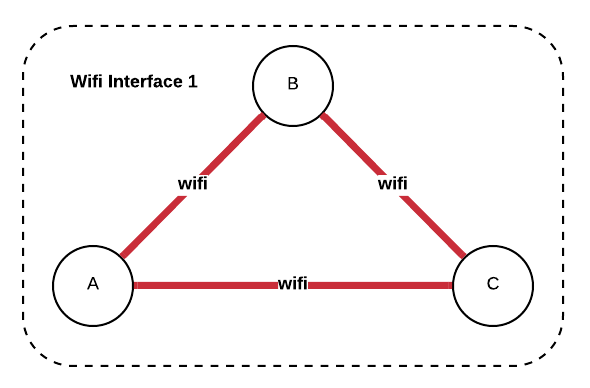
\includegraphics[width=14cm,height=20cm,keepaspectratio]{Figures/networkWifiInterface1.png}
        \caption{Network topology without defining interfaces}
        \label{fig:networkWifi1}
    \end{centering}
\end{figure}


In the Serval-DNA test framework, non- fully-connected WiFi networks are created by manually defining the WiFi interfaces that a specified Servald interface is connected to.
To implement this, several changes need to be made.
The first is removing the functions added in the previous section that relate to WiFi.
This is because we'll no longer be defining WiFi nodes with a string passed to the setup functions.
Next, it was decided for every node to automatically have WiFi functionality enabled by default, but only connected to its own private interface as this more accurately represents how real Serval nodes will act in real usage \todo{ref}.
This is done by changing the configuration parsing added in the previous section to enable WiFi by default, but still only enabling LBARD as specified.

To connect nodes via WiFi they must now be connected to a specific WiFi interface as shown in \figurename{ \ref{fig:definingInterfaces}}.


\lstset{language=bash,
showstringspaces=false,
numbers=left,
}

\begin{figure}
    \begin{centering}

        \begin{lstlisting}[breaklines, frame=single]
doc_DualType="A 4 node wifi/rfd900 chain. One wifi, two radio links"
setup_DualType(){
    # A -r-> B -w-> C -r-> D
    # No radio connection between 1(B) and 2(C)
    lbardparams="allow between 0,1; allow between 2,3; deny all;"

    setup 0 0 0 "\${lbardparams}"
    # Connect 1(B) and 2(C) via a wifi/rhizome interface of number 1
    foreach_instance +B +C add_servald_interface 1

    # Insert a file to server A
    set_instance +A
    rhizome_add_file file1 50
}
test_DualType(){
    dReceivedBundles() {
        bundle_received_by $BID:$VERSION +D
    }
    wait_until --timeout=60 dReceivedBundles
}
        \end{lstlisting}
        \caption{Example of LBARD test definition}
        \label{fig:definingInterfaces}
    \end{centering}
\end{figure}

When a node is connected to multiple nodes at once, it will be able to communicate with all other nodes in those interfaces, while the connected nodes are still only able to communicate with nodes in the same interfaces as themselves.
This means that previously impossible network topologies such as WiFi chains can be implemented as shown in \figurename{ \ref{fig:networkWifi2}}.
\todo{Fix this, it doesn't actually show what it says}

\begin{figure}
    \begin{centering}
        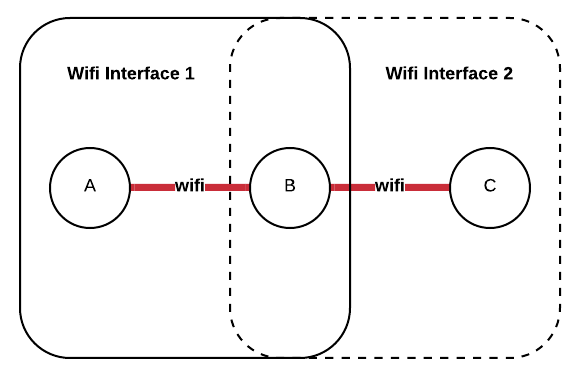
\includegraphics[width=14cm,height=20cm,keepaspectratio]{Figures/networkWifiInterface2.png}
        \caption{Network topology with two WiFi interfaces defined}
        \label{fig:networkWifi2}
    \end{centering}
\end{figure}


\section{Implementing easier network definition}
\begin{itemize}
    \item Add ability to define {n} things
    \item Add ability to define multiple radio types easily.
\end{itemize}

To assist with creating complex network topologies, a function \verb|setupN| was implemented that allowed for an arbitrary number of Servald and LBARD instances to be created and networked together.
This function is needed as the LBARD test framework lacked any way of defining an arbitrary number of Servald nodes and instead only provides function to start 4 or 8 Servald devices.
As such, a function that can create and start an arbitrary number of nodes is crucial for the expansion of the LBARD test framework.

This \verb|setupN| function accepts four parameters; a string of node characters, a string of radio types ('none' if LBARD is not to be started on the relevant node), the Fakeradio parameters (i.e. packet loss), and finally the parameters for each LBARD instance.
This function then starts a Servald process on each of these nodes, and if defined in the string of radio types, starts LBARD on the same node.
Once Servald and LBARD is running on every relevant node with the appropriate configurations as outlined in the previous sections, the function then starts \verb|fakeradio| as necessary.

With this function implemented, the testing capabilities of the LBARD test framework have dramatically increased.
By using this function, testers are able to easily define and test the exact number of Serval nodes that they require in their test, and with the capability to define exact parameters of the test — such as defining which radio to use on a per-node basis and packet loss — this relatively simply function presents a huge increase in testability.
Furthermore, this function when combined with the implementation of mixing WiFi and Fakeradio interfaces allows for Serval testers to test a far greater number of Serval networks with ease.


\section{Adding more topologies tests}


\begin{itemize}
    \item List the ones that existed previously — only used for development
    \item We need more than just the basic ones defined earlier
    \item Not just WiFi/radio
    \item Complicated topologies (find some that represent real models and reference)
\end{itemize}

\section{Summary}
\begin{itemize}
    \item Summarise what this chapter did
    \item Talk about why it was important
    \item Link to next section
\end{itemize}
\todo{Add summary}